% @Author: AnthonyKenny98
% @Date:   2020-03-01 18:51:24
% @Last Modified by:   AnthonyKenny98
% @Last Modified time: 2020-03-01 19:39:08
\subsection{RV32I}

        The following is an excerpt from the RISC-V Specification, outlining the RV32I base integer instruction set \cite{Waterman2019}
        \begin{quote}{}
            \small{RV32I was designed to be sufficient to form a compiler target and to support modern operating system environments. The ISA was also designed to reduce the hardware required in a minimal implementation. RV32I contains 40 unique instructions, though a simple implementation might \dots [reduce] base instruction count to 38 total. RV32I can emulate almost any other ISA extension \dots \\
            Subsets of the base integer ISA might be useful for pedagogical purposes, but the base has been defined such that there should be little incentive to subset a real hardware implementation \dots}
        \end{quote}

        \subsubsection*{Registers}
        RV32I defines 32 unprivileged registers, each 32 bits wide. They are designated \texttt{x0-x31}, where \texttt{x0} is a hard-wired value of $0$, and registers \texttt{x1-x31} hole values that various instructions use. RISC-V uses the load-store method, meaning that all operations perform on two registers or a register and an immediate, rather than performing operations directly on memory addresses. In addition, the 33rd unprivileged register is the program counter \texttt{pc}. Table \ref{table:rv32i_reg} shows the register state for the RV32I Base Integer Instruction Set.
        % @Author: AnthonyKenny98
% @Date:   2020-03-01 18:36:35
% @Last Modified by:   AnthonyKenny98
% @Last Modified time: 2020-03-01 19:33:20
\begin{table}[H]
\begin{center}
\begin{tabular}{|p{.15\linewidth}|p{.15\linewidth}|p{.4\linewidth}|}
    \hline
    \textbf{Register}   & \textbf{ABI Name}  & \textbf{Description} \\
    \hline
    \texttt{x0}  & \texttt{zero} & Hard-wired zero \\
    \texttt{x1}& \texttt{ra}& Return address\\
    \texttt{x2}& \texttt{sp} & Stack pointer\\
    \texttt{x3}& \texttt{gp}&Global pointer\\
    \texttt{x4}& \texttt{tp}& Thread pointer\\
    \texttt{x5-7}& \texttt{t0-2}&Temporaries\\
    \texttt{x8}& \texttt{s0/fp}&Saved register/Frame pointer\\
    \texttt{x9}&\texttt{s1} &Saved register\\
    \texttt{x10-11}&\texttt{a0-1}&Function arguments/return values\\
    \texttt{x12-17}&\texttt{a2-7}&Function arguments\\
    \texttt{x18-27}&\texttt{s2-11}&Saved registers\\
    \texttt{x28-31}&\texttt{t3-6}&Temporaries\\
    \hline
    \texttt{pc} & \texttt{pc} & Program counter \\
    \hline
\end{tabular}
\caption{Register State for RV32I Base Instruction Set}
\label{table:rv32i_reg}
\end{center}
\end{table}

        \subsubsection{Instruction Formats}
        Table \ref{table:rv32i_instr_format} demonstrates the format of each different instruction type. 
        % @Author: AnthonyKenny98
% @Date:   2020-03-01 19:13:03
% @Last Modified by:   AnthonyKenny98
% @Last Modified time: 2020-03-01 19:32:00
\begin{table}[H]
\begin{center}
    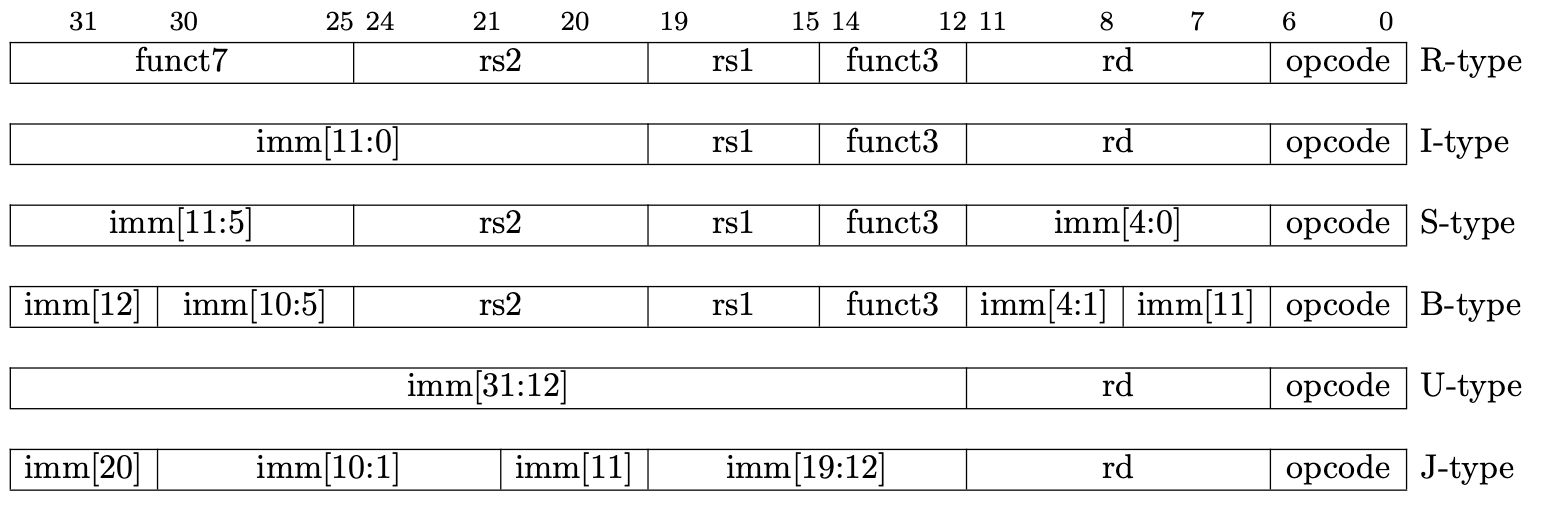
\includegraphics[draft=false,width=\linewidth]{chapters/chapter4/img/rv32i_instr_format.png}
    \caption{RV32I Base Instruction Formats}
    \label{table:rv32i_instr_format}
\end{center}
\end{table}



    \subsection{Motion Planning Extension}
        \todo[inline, caption={Motion Planning Extension}]{Full description of design of Non standard extension for motion planning. Should follow define, design, build, measure, analyse etc format.}